%-------------------------------------------------------------------------------
% COGNITIVE MEMORY
%-------------------------------------------------------------------------------
\subsection{``Cognitive" memory}
\begin{frame}{Introduction}{``Cognitive" memory}


\begin{block}{Problematic}
{
How can FCA  optimise a \textbf{cognitive} memory structure?
}
\end{block}

\vfill

\begin{block}{``Cognition"}
{
  The mental action or process of \textbf{acquiring knowledge} and 
  understanding through \textbf{thought}, \textbf{experience}, and the 
  \textbf{senses}.
}
\vfill
\hspace*\fill{\small--- Oxford Dictionary}
\end{block}

\end{frame}

%-------------------------------------------------------------------------------
% INDUCTIVE REASONING
%-------------------------------------------------------------------------------
\subsection{Inductive reasoning}
\begin{frame}{Introduction}{Inductive reasoning}

Unfamiliar objects are evaluated thanks to familiar attributes\ldots
\vfill
\begin{figure}[ht]
% KITTEN
\begin{minipage}[b]{0.2\linewidth}
\centering
\includegraphics[width=\textwidth]{img/introduction/kitten.png}
\\{\color{green}+100}
\end{minipage}
\hfill
% SEA URCHIN
\begin{minipage}[b]{0.2\linewidth}
\centering
\includegraphics[width=\textwidth]{img/introduction/urchin.png}
\\{\color{red}-100}
\end{minipage}
\hfill
% KOALA
\begin{minipage}[b]{0.2\linewidth}
\centering
\includegraphics[width=\textwidth]{img/introduction/koala.png}
\\?
\end{minipage}
\hfill
% ECHIDNA
\begin{minipage}[b]{0.2\linewidth}
\centering
\includegraphics[width=\textwidth]{img/introduction/echidna.png}
\\?
\end{minipage}

\end{figure}
\end{frame}

%-------------------------------------------------------------------------------
% SYTEM LIMITATIONS
%-------------------------------------------------------------------------------
\subsection{Bias}
\begin{frame}{Introduction}{Bias}

\ldots{}but beware of certain attribute combinations!
\vfill

\begin{figure}[ht]
% COFFEE
\begin{minipage}[b]{0.26\linewidth}
\centering
\includegraphics[width=\textwidth]{img/introduction/coffee.png}
\\{\color{green}+100}
\end{minipage}
\hfill
% LAPTOP
\begin{minipage}[b]{0.26\linewidth}
\centering
\includegraphics[width=\textwidth]{img/introduction/laptop.png}
\\{\color{green}+100}
\end{minipage}
\hfill
% COFFEE ON LAPTOP
\begin{minipage}[b]{0.26\linewidth}
\centering
\includegraphics[width=\textwidth]{img/introduction/coffee_on_laptop.png}
\\?
\end{minipage}
\end{figure}

\end{frame}

%-------------------------------------------------------------------------------
% HOW FCA CAN HELP
%-------------------------------------------------------------------------------
\subsection{How FCA can help}
\begin{frame}{Introduction}{How FCA can help}

\begin{figure}[ht]
\begin{minipage}[t]{0.55\linewidth}
\vspace{0pt}
\centering
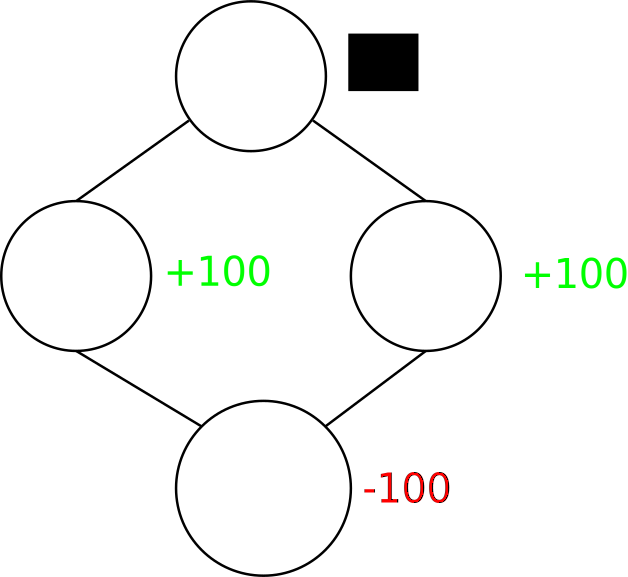
\includegraphics[width=\textwidth]{img/introduction/fca_coffee.pdf}
\end{minipage}
\hfill
\begin{minipage}[t]{0.40\linewidth}
\vspace{0pt}
\begin{block}{``Concept Lattice"}
\begin{itemize}
\item object nodes,
\item attribute nodes,
\item \underline{composite nodes},
\item \underline{abstract nodes}.
\end{itemize}
Evaluate concepts, not just objects and attributes.
\end{block}
\end{minipage}
\end{figure}

\end{frame}